\section{Bot-So}\label{s:Bot-So}

Das Bot-So Projekt ist ein \ac{IoT}-Roboter, der sich aus einem Raspberry Pi, Oracle Java SE Embedded 8, einem Bewegungssensor, einer Videokamera und einem Anschluss an den Kurznachrichtendienst Twitter zusammensetzt. Ziel ist es, Benutzern zu ermöglichen, ihr Zuhause oder ihre Arbeitsstelle zu überwachen, während sie selbst nicht anwesend sind. Die Kamera ist an einem Schwenkarm befestigt, der durch Rotationen einen Blickwinkel von $120^\circ$ ermöglicht. Um Sprachausgabe zu ermöglichen, besitzt der Roboter eine kleine Soundkarte, an die ein Lautsprecher angeschlossen werden kann. Dies ermöglicht das Wiedergeben von zuvor aufgenommenen Nachrichten\cite{ws:botsovoice}. Über Ethernet oder WLAN kann sich der zugrundeliegende Raspberry Pi mit dem Internet verbinden. Die für das komplette System benötigte Energie wird über USB geliefert.\\
Der Roboter kann entweder direkt angewiesen werden, einen Raum zu scannen und Videomaterial an den Besitzer zu senden, oder im Überwachungsmodus operieren. In diesem Modus  werden Bilder oder Videos aufgenommen, sobald der Bewegungssensor anschlägt\cite{z:botso}.\\

\begin{figure}[H] 
	\centering
	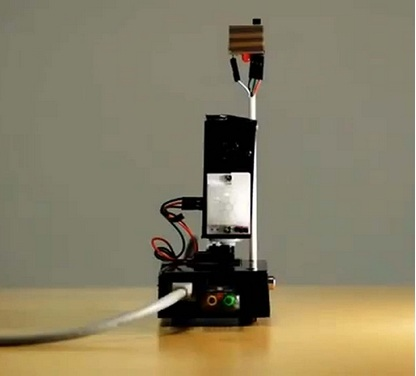
\includegraphics[scale=1.3]{Bilder/botso}
	\caption{Der Bot-So Roboter\cite{i:botso}}
	\label{f:botso}
\end{figure}

Auf dem Raspberry Pi arbeitet die weit verbreitete Debian Linux Version Raspbian, die mithilfe von Jetty, Log4j, Google Drive APIs und Java Mail die Kommunikation zum User aufnimmt. Um mit Twitter zu interagieren, bedient das Bot-So Projekt der Twitter4j Bibliothek. 

Die Kommunikation mit dem Roboter ist nahezu intuitiv. Er reagiert auf Twitter-Nachrichten wie 'Temp', woraufhin er die aktuelle Umgebungstemperatur mitteilt. 
Um einen Blick in die Umgebung des Roboters zu werfen, kann man sich entweder dem Tweet 'Take 3' bedienen, oder auf 'Sweep Room' ausweichen. Während bei 'Take 3' drei Bilder mit verschiedenen Ausrichtungen aufgezeichnet werden, fährt der Schwenkarm des Roboters bei 'Sweep Room' einmal von links nach rechts durch den Raum und zeichnet dabei ein Video auf. 
Die Dateiübertragung erfolgt über Google-Drive. Nach erfolgreichem Aufzeichnen von Video- oder Bildmaterial wird dies von dem Roboter an Google übertragen und ein Link an den Besitzer getwittert.\\


Das Robotersystem wurde von den Indern Debraj Dutta, Avinaba Brandhu Majumder, Tapas Bose und Suddhantha Krishan entwickelt. Zusammen haben sie die IoT Developer Challenge gewonnen und daraufhin die Java-One Messe besucht, um ihr Projekt vorzustellen.\\

Die Entwickler haben sich dazu entschieden, bei der Entwicklung des Projekts nur auf Open-Source Ressourcen zuzugreifen. Aufgrund dessen kann der Bot-So Roboter von jedem Bastler nachgebaut werden. Die Software hierzu kann auf Github heruntergeladen werden.
